\documentclass[dvips,12pt]{article}

% Any percent sign marks a comment to the end of the line

% Every latex document starts with a documentclass declaration like this
% The option dvips allows for graphics, 12pt is the font size, and article
%   is the style

\usepackage[pdftex]{graphicx}
\usepackage{url}
\usepackage[pdftex]{xcolor}
\usepackage{amsmath}

% These are additional packages for "pdflatex", graphics, and to include
% hyperlinks inside a document.

\setlength{\oddsidemargin}{0.25in}
\setlength{\textwidth}{6.5in}
\setlength{\topmargin}{0in}
\setlength{\textheight}{8.5in}

\newcommand{\comment}[1]
{{\bfseries \color{red} #1}}


%----------------------------------------------------------------------------------------
%	DOCUMENT INFORMATION
%----------------------------------------------------------------------------------------

\title{2016 RPA Narrative RPA-16-10565\\
Uncertainty Propagation for Fuel Cycle Calculations}

\begin{document}
\noindent\textbf{Technical Workscope Identifier:} FC-5.1b\\
\textbf{Time Frame:} 3 years\\
\textbf{Estimated Cost:} \$800,000\\


\section{Proposed Scope/Context Description}
The fuel cycle simulation tool can have a large
scope of application, from the study of the
behavior of some type of fuel or reactor inside an
existing nuclear fleet to the prospective analysis
of a complete nuclear transition. Beside the study
of fleet evolution it can also been used to assess
the possibility of material hijacking in the
context of non-proliferation study or
policy...\\ Each application field of the nuclear
fuel cycle calculation requires a specific level
of confidence, which are up to now very
un-precisely assessed, if assessed. There is a
real need of validation the those kind of
calculation, which can hardly been
reached. Indeed, the only existing way to validate
any fuel cycle calculation/tool, is the benchmark
with other similar tools, or other existing
data... When the first is generally conclude with
a list of why the different softwares end up with
different results (without concluding on the
precision of any), the second allow only the
validation on existing concept and have no impact
on calculation implying the use of new
concept.\\ The aim of this project is to add error
propagation capability to the CYCLUS fuel cycle
simulator [1]. By their usage for predicting the
evolution of a large industrial enterprise in an
uncertain future, nuclear fuel cycle simulations
are generally based on approximations and
uncertain input data.  Since validation is largely
considered to be impractical, such simulations are
seen as indications of future behavior rather than
predictions of that behavior. \\ Nevertheless, it
would be valuable to be able to place some
confidence bounds on those indications, both to
assess the robustness of conclusions that derive
from those indications and to provide information
about the sensitivity of those conclusions to the
uncertain data and algorithms.\\ Having a broad
distribution for each metric calculated in a fuel
cycle simulation instead of unique values will
allow a better comparison between different fuel
cycle scenarios.\\ Moreover for some critical
analysis such as retrospective non-proliferation
analysis, it could be extremely valuable to add
some degree of confidence on the simulation
performed. This could allow at least to confirm or
invalidate the possibility to use those
calculation tools for such purpose.\\ This project
will extend the Cyclus concept of resources to
include error information and then develop a
number of archetypes that can perform operations
to propagate that error in a rigorous fashion.
Ultimate calculation of fuel cycle performance
metrics will also need to be updated in order to
represent final results as distributions rather
than single values.

\section{Logical Path to Work Accomplishment}
The goal of this project is to add optional
extensions to Cyclus that will allow an assessment
of the error as it propagates through a fuel
cycle.

\subsection{Add uncertainty to ressources}
The first step of this work, is to update the
principal CYCLUS metric : the material and
associate the isotopic composition with a
uncertainty. 

Because of the present of cycle in a fuel cycle
calculation, one major problem could be redundancy
of certain error/uncertainty, which are related,
and should be taken into account in the
uncertainty propagation. This should require a
tracking of the error/uncertainty/tolerance source
on each material circulating inside the fuel cycle
calculation. Unfortunatly this is far to
complicated for a first step into error
propagation, therefore the uncertainty on the
material independent of any previous operation on
this materials.\\
\comment{bam: the uncertainty of a material will
be considered as independant of any error source
in a archetypes}

\comment{bam: not sure but if a composition vector
in Cyclus represents a relative composition then
one should have 2 kind of unertainty on a material
: the error on the relativ composition and the
error on the quantity on this material. Moreover
on should also have some equation which bound the
relativ uncertainty, like: \\
\begin{eqnarray}
\left\{
\begin{aligned}
&\sum_i N_i \{\delta N_i\} = 1 \{0\}\\
&\delta Q\\
\end{aligned}
\right.
\end{eqnarray}
where ${x}$ represent the uncertainty on the parameter.
}
\subsection{Archetypes uncertainty management}
In a fuel cycle calculation, there are three
different uncertainty/error sources :
\begin{itemize}
\item the material uncertainty,
  $\delta\vec{N}_{in}$, which is the input and the
  output of each archetypes,
\item the "tolerance", $\tau_{i}$, on the input
  parameter, which corresponds the possible
  variation range of any physics parameter, $i$,
\item the error, $\epsilon_{mod}$, introduce by
  the archetypes modeling/operation on the
  material.
\end{itemize}
The uncertainty on the output material is a
function of all those uncertainties :
\begin{equation}
\delta \vec{N}_{out} = {\cal F}\{~\delta\vec{N}_{in}~,~\tau_0~,~...~,~\tau_n~,~\epsilon_{mod}~\}
\end{equation}
The work we are proposing to do on this project,
is to allows all archetypes of CYCLUS, to combine
all those sources and computes the resulting
uncertainties on the output materials.  In the
following parts, one will tried to detail the work
which need to be done on the different archetypes,
we are proposing to update.
\subsubsection{Enrichment facility}
The enrichment facility is probably the easiest
facility to model, since the only error come from
the tails and feed stream enrichments, the
enrichment process could be linearly models. This
can be easily analytically combine and propagate.

%\footnote{note that in this case the feed stream
%enrichment can be also see as incoming material
%uncertainty.}:

%\begin{equation}
%\forall i, \left(\frac{\delta N_{i}}{N_{i}}\right)^{2}_{out} = \left(\frac{\delta N_{i}}{N_{i}}\right)^{2}_{in} +  \left(\frac{\tau e_{tails}}{e_{tails}}\right)^{2} 
%\end{equation}

\textit{Is it true with any enrichment technic ?}

\textit{do we want the exact error propagation formula ?}

\subsubsection{Separation}
As the enrichment process, the separation should
be very easy to model including
uncertainty. Indeed, the only parameter which can
introduce extra variance is the separation
efficiency, $\tau_{eff}$.

% Since the uncertainty on the input material and
% the tolerance of the efficiency is independent
% (supposed gaussian) , the resulting uncertainty
% on the output material composition can express
% as :

%\begin{equation}
%\forall i, \left(\frac{\delta N_{i}}{N_{i}}\right)^{2}_{out} = \left(\frac{\delta N_{i}}{N_{i}}\right)^{2}_{in} +  \left(\frac{\tau s_{eff}}{s_{eff}}\right)^{2} 
%\end{equation}

\textit{do we want the exact error propagation formula ?}

\subsubsection{Reactor}
As all archetypes the reactor, are subject to
physical parameter fluctuation.The different
parameter one should consider are the discharge
burnup, the effective power/capacity
factor... Variation consideration on those
parameters will affect the discharge time, which
should be very difficult to include in the
uncertainty calculation. Nevertheless, a brute
force study ( also sometimes called "Total Monte
Carlo method") could allow the determine their
impact, running many time the same simulation
choosing randomly the parameter value at each
cycle of the reactor, the distribution of the
results will provides a precise measurement of the
sensivity.\\

We are envisaging two kind of the reactor, which
will be both capable to handle uncertainty. The
first one will be built as an upgrade of the
existing CYCAMORE reactor, making it error
aware. The CYCAMORE reactor is a recipe base
reactor, in addition of all the classical reactor
parameter (batch number, cycle length, power,
capacity factor,...) the user provides the input
and output fuel recipes. The only requirement is
to force user to provide the output recipe with
the according sensitivity to input
uncertainty. From this sensitivity, one will be
able to compute directly the output uncertainty on
the output composition from the input one.\\

%\begin{equation}
%\forall i, \left(\frac{\delta N_{i}}{N_{i}}\right)^{2}_{out} = \left(\frac{\delta N_{i}}{N_{i}}\right)^{2}_{in} +  \left(\frac{\tau s_{eff}}{s_{eff}}\right)^{2} 
%\end{equation}

The second version of reactor will be able to
calculate the evolution of the fuel provided by
the fuel fabrication (see \S
\ref{sec:fabrication}).  To do so, we propose
investigating two ways, both using pre-trained
models, allowing the prediction of key physics
parameters needed to compute the evolution of a
fuel during the irradiation. It has been proven
that from pre-trained neural network models, one
can predict the evolution of the one group cross
section during the irradiation of the fuel from
its initial isotopic composition, and is working
for a various range of reactor, from LWR to SFR
\cite{Leniau Neural networks,
  Leniau.PHYSOR.2016}.\\ 
The first application using the neural network
predictive models, is to train a model to directly
predict the composition evolution as the function
of the burnup. This application might not work,
since the usage of neural network has been proven
to predict one group macroscopic cross
section.\\ 
If the neural network model fail to directly
predict precisely the isotopic composition
evolution, one have to consider the second option,
which imply to predict the 1 group cross section,
then integrate the Bateman equation.\\

The main reason leading the try of direct
prediction of the isotopic evolution, is the
error/uncertainty propagation. As express
prevsiously :

\begin{equation}
\delta \vec{N}_{out} = {\cal F}\{~\delta\vec{N}_{in}~,~\tau_0~,~...~,~\tau_n~,~\epsilon_{mod}~\}
\end{equation}
The determination and the propagation of all
uncertainty source is, for this kind of reactor, a
complicated matter. The error due to the
computation of the depletion calculation are wild:
\begin{itemize}
\item the error of the neural network predictor,
  $\epsilon^{nn}_{i}$, with $i\in[0..N]$, $N$ the
  number of predicted parameter,
\item the convolution of the uncertainty on the
  material composition with the neural network
  prediction.
\item the calculation error on the data sets used
  to train the neural network, $\epsilon_{T.D.}$.
\end{itemize}
And then can be expressed as :
\begin{equation}
\epsilon_{mod} = {\cal G}\{~\delta\vec{N}_{in}~,~\epsilon^{nn}_{0}~,~...~,~\epsilon^{nn}_{n}~,~\epsilon_{T.D.}~\}
\end{equation}

Because, the predictive model are trained on
sample populated using few thousand of depletion
calculation, which are subject to computation
error, $\epsilon_{T.D.}$. On one side, a depletion
calculation take as input, the nuclear data. Those
nuclear data are interpolated/extrapolated from
many different experimental measurement using many
different models. Therefore the nuclear data
contain uncertainty...  Those uncertainty are
extremely difficult to propagate properly through
a full depletion calculation because of the
coupling between neutron transport and depletion
calculation: the composition of the fuel impact
the shape of the neutron spectrum, which impact
the reaction rate on the nuclei... On the other
side, the depletion calculation require different
approximation to be completed. There is nearly
impossible using Monte Carlo technique on a PWR
full core calculation due to source convergence
issue. It is also extremely complicate to follow
precisely the different reactor parameter, such as
boron concentration, rod control management,
charge factor evolution, neutron leakage... The
study and the propagation of the modeling
uncertainty, such as the modeling simplification
and the nuclear data uncertainty is way beyond the
scope of this project...\\ 
This require a full dedicated research project
(and probably more). Therefore, those error,
$\epsilon_{T.D.}$, will not be considered on the
first version of this work. This might need to be
reconsidered when the depletion calculation error
propagation capacity will have done important
progress.\\
The direct error induced by the use of predictive
model, $\epsilon^{nn}_{i}$ on each parameter, $i$,
need to be assessed. This could be performed with
a mapping the error on the isotopic space
populated with the training sample. This will
allow to determine the error of the model on each
point on the isotopic space populated. We might
use then a other neural network, or other
interpolation method to predict the error of the
prediction as the function of the isotopic
composition.\\
Once we have a working predictive model and a map
of the error on the prediction, one need to build
the covariance matrix which will allow to
convolute the uncertainty on the input material,
$\delta N_{in}$, with the prediction of the
model.\\


If the direct prediction of the composition is not
precise enough, one have to use solve Bateman
equation using predicted one group cross section
and then compute the error coming from a numerical
resolution of the Bateman equation and propagate
the error of the one group cross section.  The
Bateman equation resolution will be a step by step
process. After having discretize the irradiation
time (or burnup), one will use the model to
predict the cross section at each time step
(closer the time step are preciser the calculation
will be) and then solve numerically the Bateman
equation step after step, ending with the final
isotopic composition of the fuel. Because the
predictive model will be able to predict the one
cross section as the function of time (or burnup),
one should be able to propagate those error using
sensitivity analysis.  The time discretization as
well as the other approximation require to solve
the Bateman equation will also introduce
computation error that need to be determined and
added to the final uncertainty. This could be made
with the comparison of depletion calculation made
with those extra approximation with the reference
one performed using the same modeling
approximation as the training depletion all along
the isotopic space.



\subsubsection{Fabrication} \label{sec:fabrication}
The aim of the fuel fabrication is to mix
different incoming material streams in order to
build a fuel which validate the neutronics/physics
requirement of the reactor. Depending of the
reactor, the criterium could be various. We are
considering in the first time including
fabrication model for MOX fuel only, in LWR and
SFR, used as burner and breeder for SFR. One will
use algorithm building fuel allowing to build fuel
reaching the targeted burnup according to either
criticality criterium either conversion ratio
criterium.  Those algorithm will relies on the
capabilities of some predictive model to predict
the maximal achievable burnup depending on the the
criticality or conversion ratio evolution
according to burnup.  The predictive model as the
reactor model, will be based on the use of neural
network formerly trained on the same set of
training depletion calculation used for the
reactor models. The capability of the neural
network have been proven to predict the evolution
of the criticality in PWR reactor using MOX fuel
\cite{Leniaux.NN, CLASS_UserManual}, as well as
the the initial criticality of MOX fuel in SFR
\cite{CLASS UserManual} and should be possible to
extend it to conversion ratio evolution.

The error/uncertainty propagation for fuel
fabrication should be pretty similar than for
reactor. Indeed the uncertainty can be expressed
as :
\begin{equation}
\delta \vec{N}_{out} = {\cal H}\{~\delta\vec{N}_{in}~,~\epsilon_{mod}~\}.
\end{equation}
In this case there is no tolerance, since the
parameter are goal to achieve, not physicals
characteristics. As well as previously the error
of the model can be expressed as :
\begin{equation}
\epsilon_{mod} = {\cal K}\{~\delta\vec{N}_{in}~,~\epsilon^{nn}_{0}~,~...~,~\epsilon^{nn}_{n}~,~\epsilon_{T.D.}~\},
\end{equation}
 where $\epsilon^{nn}_{i}$ represent the error on
 the prediction of the parameter $i$ by the neural
 network predictive model and $\epsilon_{T.D.}$
 the error due to the error on the depletion
 calculation composing the training set, which
 will not be considered since we dont have any way
 to correctly estimate it.\\
 
 As for the reactor model, the $\epsilon^{nn}_{i}$
 component of the error can be determined through
 a mapping of the error along the isotopic space,
 and the impact of the material input uncertainty
 needed the be assessed by the calculation of the
 covariance matrix which need to be build.

\subsection{Problems/Applications/Validations}
During the realization of this work we would like
to validate each step of the uncertainty
propagation process. First, with a mid/early-term
validation, after the enrichment facilities, the
separation and the recipes reactor will be
implemented, it will be possible to confirm the
uncertainty is correctly propagated, using a brute
force validation (with the "Total Monte Carlo"
method). This validation will be continued with
new archetypes will be implemented in CYCLUS...\\
An other gaol we want to achieve, is an
sensitivity analysis, allowing to determine the
impact of the different
uncertainty/error/tolerance on the final
calculation uncertainty. This should allow to
define precisely where the future effort should be
focus to reduce those uncertainty sources
accordingly to the object of the calculation and
also to validate (or un-validate) the use of fuel
cycle simulation tool for some specialized study
(such as non-proliferation study...)\\
With all the necessary components in place, a
series of demonstration simulations will be
conducted using fuel cycles of increasing
complexity: once through, MOX LWR recycle, and
fast reactor recycle.  These scenarios will be
constructed to highlight the role of error and
uncertainty and identify metrics in which the
presence uncertainty may impact fuel cycle
analysis conclusions.



%\textit{We imagine 3 step in the final
%phase. First we would like to step up a testing
%mechanism, based on simply brute force the
%uncertainty propagation in the fuel cycle
%calculation by using some kind of Total monte
%Carlo, allowing all parameters to fluctuate
%accordingly to their respective uncertainty on
%many integration of the same calculation. The
%result distribution can be read as a direct
%measure of the uncertainty on the final parameter
%and will be compared to the direct uncertainty
%propagation calculation as a validation of all
%the method previously presented. This method will
%(turning on the uncertainty on each parameter one
%by one) to validate the uncertainty propagation
%on each parameter...\\

%One need nevertheless keep in mind that
%everything is never perfect, and one should
%always try to improve. To do so it is required to
%identify the most problematic issue and solve
%it. In this particular case, one need to identify
%what is the uncertainty gaol depending on the
%application of the fuel calculation, of course
%the precision goal is very different when one
%doing a prospective calculation versus a
%non-proliferation retrospective
%analysis... Knowing it, one very important of
%this project is it could allow through
%sensitivity analysis to identify the biggest
%uncertainty source, and help to focus to improve
%it.\\ 

%That is why, in addition of the TMC test tool, I
%would like to develop a tool/method to
%systematically allows user to perform sensitivity
%analysis applied to their calculation allowing us
%to improve future models dedicated to some
%precise use of the CYCLUS tool.\\

%Finally, we would like
%Third step : application to simple case : PWR, transition from PWR to FBR...}
\section{Relevance of Proposed Research}
This proposal aims to provide an important feature
needed in the fuel cycle simulator.  Given the
appropriate estimation of the error relative to
any fuel cycle simulation, the simulator would be
able to make decisions about fuel cycle transition
like fuel reprocessing, or the launching of new
technologies or types of reactors. Furthermore,
the project will be one of the first of its kind
to introducing error propagation in fuel cycle
calculation, increasing the utility of the Cyclus
kernel. Since the precision of fuel cycle tool
have never been assessed, this work might the
first step providing more confidence in the fuel
cycle calculation. And even if this wok will be
applied to the fuel cycle simulation tool CYCLUS,
the concept should be a theoretically applicable
on any agent based fuel cycle simulation
tool.\\ 
Additionally, new archetypes will be contributed
to the Cyclus ecosystem, including not only error
propagation but also different fuel fabrication
methods, cross-section prediction models and a
Bateman equation solver. These features will
permit future comparison between the different
fuel fabrication models and improve the user
experience and confidence in the interpretations
of Cyclus simulations.

\pagebreak
\section{Milestone Task Listing}
This research project consist in four major tasks
that could be conducted in parallel.  The first
one will be very short ($<$ 6 month), dedicated to
update CYCLUS and allow it to handle
uncertainty. The second one should be the longer
task (12 - 24 months) where the models will be
developed. The predictive model development
can/should/will be started at the start of the
project. The third will be started after the end
of the TASK 1 and corresponds to CYCLUS archetypes
update and included in a separated package. The
development of some archetypes will depends on the
progress on the TASK2. The last task is the
validation and application one and will be started
with the completion of the different
TASK3-subtasks. The ideal progression is
represented on the figure \ref{fig:progression}.
\begin{figure}[h!]
\centering
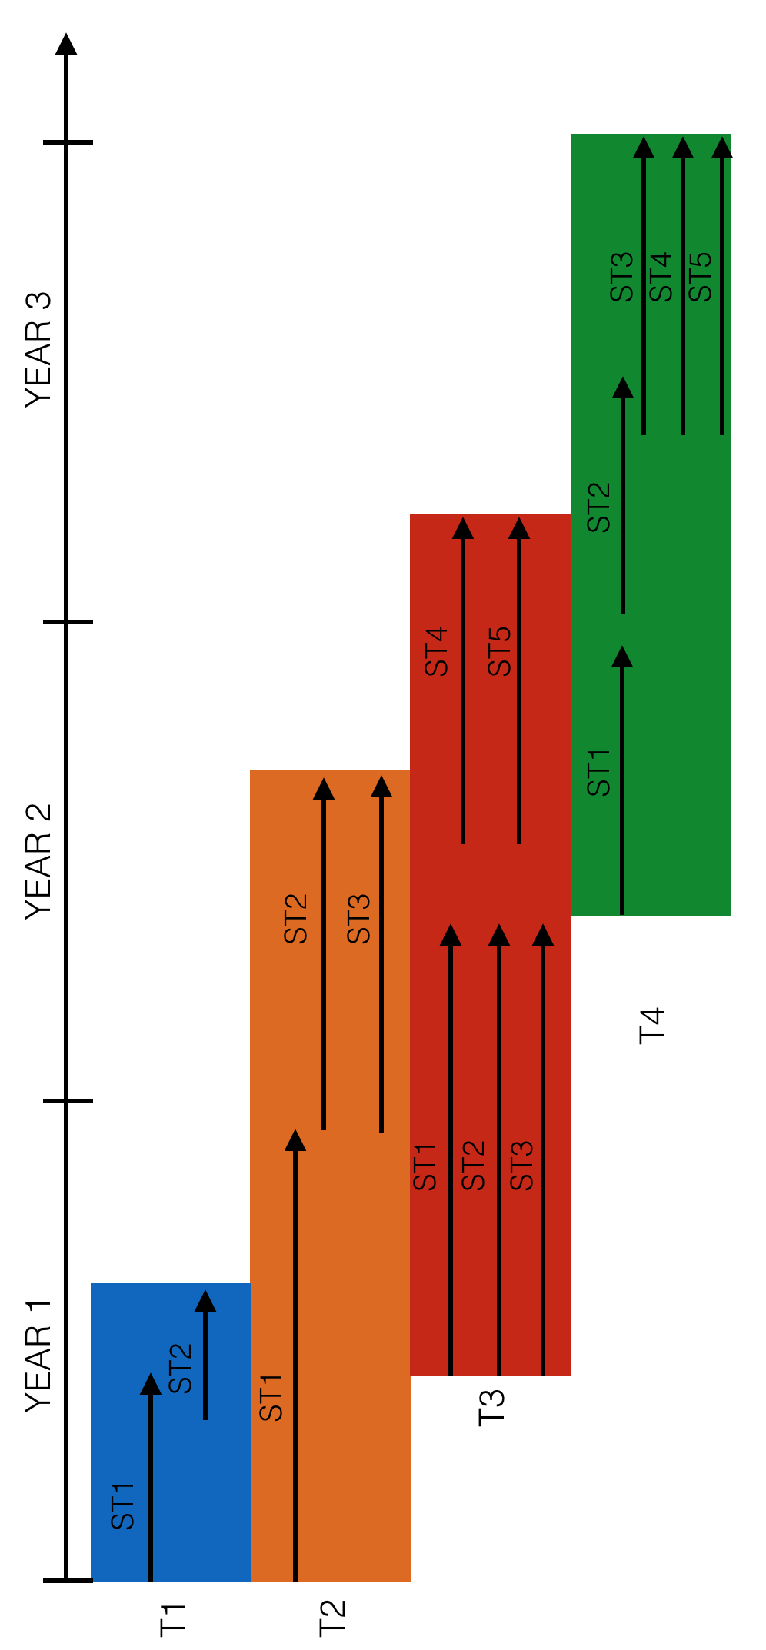
\includegraphics[angle=270,width=1\textwidth]	{TIMESCHEDULE}
\caption{Preliminary schedule of the project, with the different Task (T\#) (1 in blue, 2 orange, 3 red, 4 green) and the corresponding subtask (SB\#).}
\label{fig:progression}
\end{figure}

\noindent\textbf{TASK 1:} CYCLUS update for uncertainty awareness
\begin{itemize}
\item subtask 1: update material to uncertainty,
\item subtask 2: validate the backward
  compatibility,
\item subtask 3: Add a default uncertainty
  behavior when using both uncertainty aware
  archetypes and standard one in the same time ?
\end{itemize}

\noindent\textbf{TASK 2:} Updating the CYCLUS Archetypes to uncertainty management
\begin{itemize}
\item subtask 1: enrichment facility, 
\item subtask 2: separation facility,
\item subtask 3: recipe reactor,
\item subtask 4: reactor archetypes, depletion
  calculation/prediction, uncertainty propagation,
\item subtask 5: fuel fab archetypes, mixing
  calculation/prediction, uncertainty propagation.
\end{itemize}

\noindent\textbf{TASK 3:} Modeling development
\begin{itemize}
\item subtask 1: isotopic space definition,
  training sample realization
\item subtask 2: reactor models development:
  parameter prediction, error analysis
\item subtask 3: fuel fabrication model
  development: parameter prediction, error
  analysis
\end{itemize}
 
\noindent\textbf{TASK 4:} Validation \& application
\begin{itemize}
\item subtask 1: validation of the overall process
  with simple calculation : enrichment +
  separation + recipe reactor
\item subtask 2: validation of modeling
  capabilities (Fab + reactor)

\item subtask 3: exemple calculation: PWR,
  transition from PWR to FBR
\item subtask 4: full sensitivity analysis

\item subtask 5: time dependent parameters
  sensitivity analysis (discharge burnup, capacity
  factor...)

\item subtask X: comparison with other physic
  modeling capabilities such as Bright-Lite ?
\end{itemize}






 







%----------------------------------------------------------------------------------------
%	BIBLIOGRAPHY
%----------------------------------------------------------------------------------------

\bibliographystyle{unsrt}

\bibliography{}

%----------------------------------------------------------------------------------------


\end{document}
